We develop a control-communication control-aware approach towards scheduling in time-sensitive settings. Due to the tight latency constraints placed on the communications, we leverage knowledge of the control state and dynamics to determine a more principled and opportunistic method of scheduling devices. In particular, we use control information to identify maximum data rates we can achieve while maintaining strong control performance so as to meet latency targets. We first derive a manner in which we can evaluate control performance. Consider a quadratic Lyapunov function $L(\bbx) := \bbx^T \bbP \bbx$ for some positive definite $\bbP \in \reals^{p \times p}$ that measures the performance of a system as a function of the state. For the system to both remain stable and over time be driver to zero, it is necessary for value of $L(\bbx_{k+1})$ to decrease relative to $L(\bbx_k)$ at all times $k$. We cannot guarantee this occurs deterministically, but instead consider a condition on the estimated future Lyapunov cost, i.e.
%
\begin{align} \label{eq_lyop}
\E [L(\bbx_{i,k+1}) \mid \hbx^{(l_i)}_{i,k},\bbh_{i,k},\mu_i,\bbsigma_i) \leq \rho \E [L(\bbx_{i,k}) \mid \hbx^{(l_i)}_{i,k}] + c_i,
\end{align}
%
for some $\rho \in (0,1)$. The condition in \eqref{eq_lyop} specifies that the expected Lyapunov cost for system $i$ should decrease by a factor of $\rho$ from cycle $k$ to $k+1$ (up to constant $c_i$). Observe that this expectation is conditioned upon the estimated state $\hbx^{(l_i)}_{i,k}$, channel conditions $\bbh_{i,k}$, as well as a scheduling decision $\{\mu_i, \bbsigma_i\}$. The scheduling decision impacts this expected value through the resulting PDR $q(\bbh_i, \mu_i, \bbsigma_i)$ which determines the probability of closing the control loop and thus diminishing this Lyapunov cost. We may derive an explicit or equivalent condition on  $q(\bbh_i, \mu_i, \bbsigma_i)$ to satisfy the condition in \eqref{eq_lyop}, which we present in the following proposition. The proof can be found in \cite{EisenEtal18}.
%%%%%%%%%%%%%%%%%%%
\begin{proposition}\label{prop_pdr_constraint}
Consider the switched dynamics in \eqref{eq_control_switch}. Define the closed-loop state transition matrix $\bbA^c_i := \bbA_i + \bbB_i \bbK_i$ and $j$-accumulated noise $\omega_i^j := \Tr[(\bbA_i^T\bbP^{1/j} \bbA_i)^{j} \bbW_i]$. The control constraint in \eqref{eq_lyop} is satisfied for device $i$ if and only if the following condition on PDR $q(\bbh_{i,k},\mu_i,\bbsigma_i)$ holds, 
%
\begin{align}\label{eq_pdr_constraint}
&q(\bbh_{i,k},\mu_i,\bbsigma_i) \geq \tdq_i(\hbx^{(l_i)}_{i,k}) :=  \\ &\ \frac{1}{\Delta_i} \left[  \left\| (\bbA^c_i - \rho_i\bbI)\hbx^{(l_i)}_{i,k} \right\|_{\bbP^{\frac{1}{2}}}^2+ (1-\rho_i)\sum_{j=0}^{l_i-1} \omega_i^j + \omega_i^{l_i} - c_i  \right],  \nonumber
\end{align}
%
where we have further defined the constant
%
\begin{equation}\label{eq_noise_diff}
\Delta_i :=  \sum_{j=0}^{l_i-1}[\omega^{j+1}_i - \Tr(\bbA^{cT}_i (\bbA_i^T\bbP^{1/j}\bbA_i)^j \bbA^c_i\bbW_i)  ].
\end{equation}
\end{proposition}
%

Proposition \ref{prop_pdr_constraint} formally establishes lower bound $\tdq_i(\hbx^{(l_i)}_{i,k})$ on the PDR of device $i$ such that its Lyapunov condition in \eqref{eq_lyop} is met in expectation. This bound is determined based upon the current estimated state, overall system dynamics, and transmission history and effectively sets a constraint on the scheduling bandwidth of FD $\bbsigma_i$ and DR $\mu_i$. We point out the relevant components of the expression in \eqref{eq_pdr_constraint}. First, note that the first term on the right hand will grow larger as the state gets larger, or closer to instability. Likewise, the latter two terms on the right hand side together grow larger as the estimating noise increases due to successive dropped packets, due to both the noise variance $\bbW_i$ and last-update counter $l_i$. In this manner, it is both the current control state and transmission history, as they relate to the dynamics of the system, that set a delivery rate requirement for each device.

The PDR condition in \eqref{eq_pdr_constraint} is valuable in the time-constrained settings because it allows us to dynamically adapt the data rate needs of each device relative to their control state. While the latency requirement effectively constrains the total resources available, the ability to properly identify the users to be given scheduling slots is and important consideration in maintaining overall reliable performance. It is worth pointing out, that depending upon the system dynamics of a particular control system, the PDRs derived in \eqref{eq_pdr_constraint} may often be in practice significantly lower than the standard, fixed PDR requirements used in high-reliability systems, e.g. $\geq 0.99$. In such cases, the identification of PDR requirements necessary for proper operation of the control system can reduce a large amount of resource constraints, as is later seen in the simulations in Section \ref{sec_numerical_results}. We proceed now to discuss the ways in which the dynamic and more lenient PDR targets in \eqref{eq_pdr_constraint} may be leveraged by the scheduling to further reduce the total transmission times.

%\begin{remark}\normalfont
%It is worthwhile to note that by placing a stricter Lyapunov decrease constraint with smaller  rate $\rho_i$ in \eqref{eq_c22}, then the first term on the right hand side of \eqref{eq_pdr_constraint} also grows larger and increases the necessary PDR. Generally, selecting a smaller $\rho$ will result in a faster convergence to stability but will require stricter communication requirements. In fact, we may use the inherent bound on the probability $q(\bbh_{i,k},\mu_i,\bbsigma_i) \leq 1$ to find a lower bound on the Lyapunov decrease rate $\rho_i$ that can be feasibly obtained based upon current control state and system dynamics. This bound, however, may not be obtainable in practice due to the scheduling constraints. In practice, we select $\rho_i$ to be in the interval $[0.90,0.1)$. 
%\end{remark}

\subsection{Selective scheduling}\label{sec_rss}
We first consider a stochastically \emph{selective scheduling} protocol, whereby we do not attempt to schedule every device at each transmission cycle, but instead select a subset to schedule a principled random manner. Define by $\nu_{i,k} \in [0,1]$ the probability that device $i$ is included in the transmission schedule at time $k$ and further recall by $q(\bbh_{i,k},\mu_i,\bbsigma_i)$ to be the packet delivery rate with which it transmits. Then, we may consider the \emph{effective} packet delivery rate $\hat{q}$ as 
%
\begin{align}\label{eq_effective_pdr}
\hat{q}(\bbh_{i,k},\mu_i,\bbsigma_i) = \nu_{i,k} q(\bbh_{i,k},\mu_i,\bbsigma_i)
\end{align}
%
Observe that in order to meet the PDR target defined in \eqref{eq_effective_pdr}, device $i$ would need to meet a \emph{modified} PDR  target $q(\bbh_{i,k},\mu_i,\bbsigma_i) \geq \tdq_i(\hbx^{(l_i)}_{i,k})/\nu_{i,k}$. While imposing a tighter PDR requirement will indeed require longer transmission times, this added time cost is generally less than the transmission overhead of scheduling all users. In particular, the scheduling probability of device $i$ is defined relative to its PDR requirement $\tdq_i(\hbx^{(l_i)}_{i,k})$ as 
%
\begin{align}\label{eq_prob_c}
\nu_{i,k} := e^{\tdq_i(\hbx^{(l_i)}_{i,k})-1} .
\end{align}
%
Notice that, when a transmission is necessary, i.e. $\tdq_i(\hbx^{(l_i)}_{i,k}) = 1$, then device $i$ is included in the scheduling with probability $\nu_{i,k} = 1$.



\subsection{Assignment-based scheduling}\label{sec_assignment}

%%%%%%%%%%%%%%%%%%%%%%%%%%%%%%%%%%%%%%%%%%%%%%%%%%%%%%%%%%%%%%%%
%%%%   A   L   G   O   R   I   T   H   M   %%%%%%%%%%%%%%%%%%%%%
%%%%%%%%%%%%%%%%%%%%%%%%%%%%%%%%%%%%%%%%%%%%%%%%%%%%%%%%%%%%%%%%
{\linespread{1.3}
\begin{algorithm}[t] \begin{algorithmic}[1]
\STATE \textbf{Parameters:} Lyapunov decrease rate $\rho$
\STATE \textbf{Input:} Channel conditions $\bbh_{i,k}$ and estimated states $\hbx^{(l_i)}_{i,k}$ for all $i$
\STATE Compute target PDR $\tdq_i(\hbx^{(l_i)}_{i,k})$ for each device $i$ [cf. \eqref{eq_pdr_constraint}].
\STATE Determine selection probabilities $\nu_{i,k}$ for each device [cf. \eqref{eq_prob_c}].
\STATE Select devices $\ccalI_k$ with probs. $\{\nu_{1,k},\hdots,\nu_{m,k}\}$
\STATE Determine set of FDs/TDs $\ccalS'_k$ [cf. \eqref{eq_ru_sets}].
\STATE Determine max. DR for each device/FD assignment [cf. \eqref{eq_mcs_select}].
\STATE Schedule selected devices via assignment method \cite{kuhn1955hungarian}.
\STATE \textbf{Return:} Scheduling variables $\{\bbsigma_{i}, \mu_i, \alpha_i\}_{i=1}^m$ 
\end{algorithmic}
\caption{Control-aware scheduling for low-latency at cycle $k$}\label{alg_calls} \end{algorithm}}
%%%%%%%%%%%%%%%%%%%%%%%%%%%%%%%%%%%%%%%%%%%%%%%%%%%%%%%%%%%%%%%%

%%%%
\begin{table}[]
\centering
\begin{tabular}{|c|c|c|}
\hline 
\textbf{TD 1} & \textbf{TD 2} & \textbf{TD 3}        \\ \hline \hline
\multicolumn{1}{|c|}{FD 1} & \multicolumn{1}{c|}{\multirow{2}{*}{FD 8}} & \multicolumn{1}{c|}{\multirow{4}{*}{FD 11}} \\ \cline{1-1}
\multicolumn{1}{|c|}{FD 2} & \multicolumn{1}{c|}{}                       & \multicolumn{1}{c|}{}                       \\ \cline{1-2}
\multicolumn{1}{|c|}{FD 3} & \multicolumn{1}{c|}{\multirow{2}{*}{FD 9}} & \multicolumn{1}{c|}{}                       \\ \cline{1-1}
\multicolumn{1}{|c|}{FD 4} & \multicolumn{1}{c|}{}                       & \multicolumn{1}{c|}{}                       \\ \hline
\multicolumn{1}{|c|}{FD 5} & \multicolumn{1}{c|}{\multirow{4}{*}{FD 10}} & \multicolumn{1}{c|}{\multirow{4}{*}{FD 12}} \\ \cline{1-1}
\multicolumn{1}{|c|}{FD 6} & \multicolumn{1}{c|}{}                       & \multicolumn{1}{c|}{}                       \\ \cline{1-1}
\multicolumn{1}{|c|}{FD 7} & \multicolumn{1}{c|}{}                       & \multicolumn{1}{c|}{}                       \\ \cline{1-1} \hline
\end{tabular}
\caption{Example of FD selection with $m_k= 12$ devices. There are a total of $S_k = 3$ TDs, given $n_1=9$, $n_2 = 3$, $n_3 = 2$ FDs, respectively.}
\label{tab_rus}
\end{table}
%%%%%

  %%%%%%%%%%%%%%%%%%%%%%%%%%%%%%%%
%%%%%%%%%% F I G U R E %%%%%%%%%%%%%%%%%
%%%%%%%%%%%%%%%%%%%%%%%%%%%%%%%%
\begin{figure*}[t]
\centering
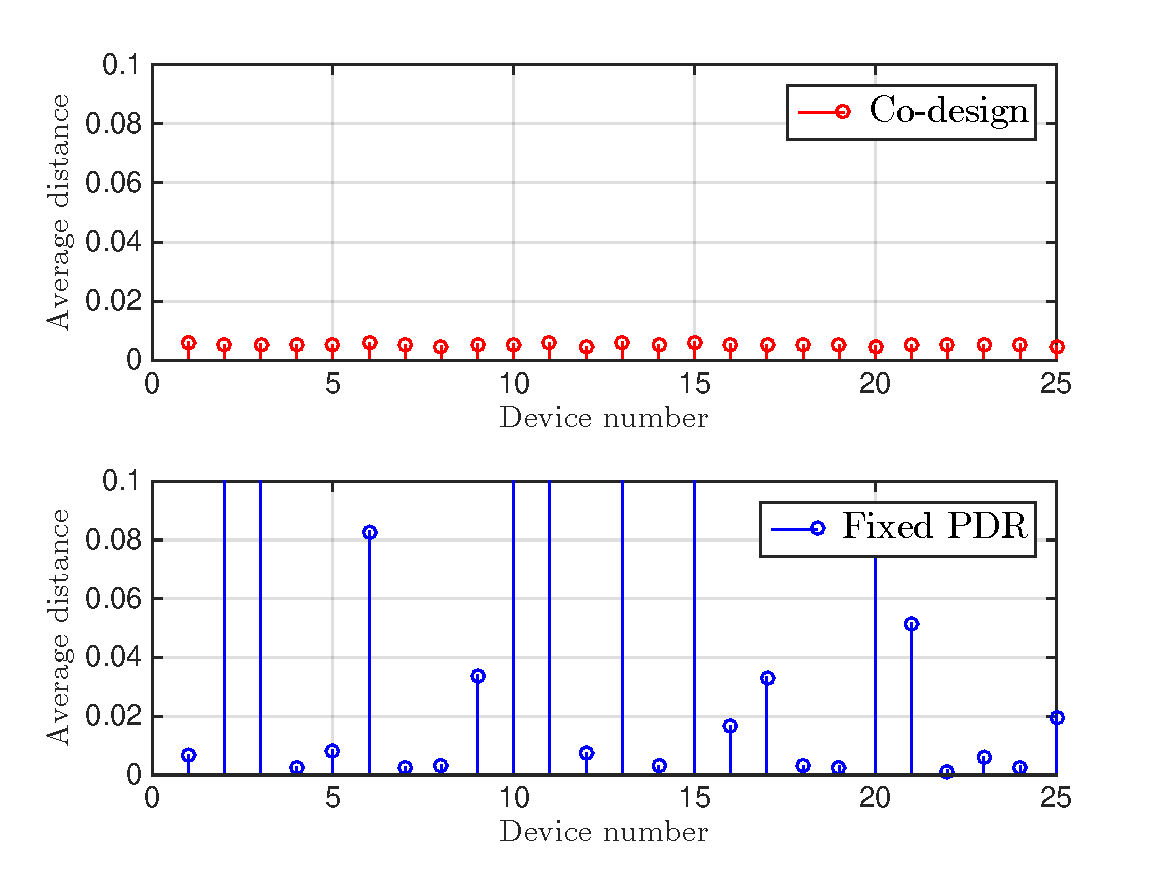
\includegraphics[width=0.4\linewidth,height=0.25\linewidth]{../images/ip_dist2.pdf} \qquad
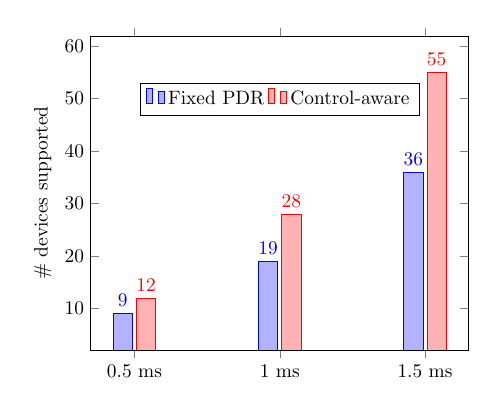
\begin{tikzpicture}[scale=0.7]
\begin{axis}[
    ybar,
    enlargelimits=0.15,
    legend style={at={(0.5,0.85)},
      anchor=north,legend columns=-1},
    ylabel={\# devices supported},
    symbolic x coords={0.5 ms,1 ms,1.5 ms},
    xtick=data,
    nodes near coords,
    nodes near coords align={vertical},
    ]
\addplot coordinates {(0.5 ms,9) (1 ms,19) (1.5 ms,36)};
\addplot coordinates {(0.5 ms,12) (1 ms,28) (1.5 ms,55)};
\legend{Fixed PDR, Control-aware}
\end{axis}
\end{tikzpicture} 
\caption{Simulation results for a series of inverted pendulums controlled over shared wireless channel. (left) The average distances from center vertical for $m=25$ pendulums. The control-aware, or ``co-design'', scheduler keeps all pendulums close, unlike the fixed PDR scheduler. (right) For different latency bounds, the control-aware can support more pendulums than the fixed PDR scheduler.}\label{fig_sim_results}
\end{figure*}


Given the set of devices selectively scheduled via \eqref{eq)prob_c}, we proceed to discuss an assignment-based formulation that can be employeed to select a low-latency schedule. Define the set of $m_k$ devices to selected be scheduled as $\ccalI_k \subseteq \{1,2,\hdots,m\}$ where  $| \ccalI_k| = m_k$ and device $j \in \ccalI_k$ with probability $\nu_{i,k}$. Further define $\ccalS_{(n)} \subset \ccalS$ to be an arbitrary set of $n$ FDs that do not intersect over any frequency bands, i.e. $\sum_{j \in \ccalS_{(n)}} \bbsigma_j \leq \mathbf{1}$. To accommodate the $m_k$ devices to be scheduled, we consider a set of $S$ such sets  $\{\ccalS^s_{(n_s)}\}_{s=1}^S$ with size $n_s$, whose combined elements total $\sum_{s=1}^{S} n_s = m_k$. We define this full set of assignable FDs at cycle $k$ as
%
\begin{align}\label{eq_ru_sets}
\ccalS'_k :=\ccalS^1_{(n_1)} \cup \ccalS^1_{(n_2)} \cup \hdots \cup \ccalS^{S_k}_{(n_{S_k})}.
\end{align}
%
Observe that an FD $\bbsigma$ is further superindexed by its TD slot $s$ y. In this way \eqref{eq_ru_sets} defines a complete set of  combinations of frequency-allocated FD and \emph{time}-allocated TDs to assign users during this cycle. An example of a possible $\ccalS'_k$ for scheduling $m_k = 12$ devices is shown in Table \ref{tab_rus}. 



For all $i \in \ccalI_k$ and FD $\bbsigma \in \ccalS'_k$, define the largest affordable DR given the \emph{modified} PDR requirement $\tdq_i(\hbx^{(l_i)}_{i,k})/\nu_{i,k}$ by
 %
 \begin{align}\label{eq_mcs_select}
 \mu_{i,k}(\bbsigma) := \begin{cases}
 \max \{\mu \mid q(\bbh_{i,k},\mu,\bbsigma) \geq \tdq_i(\hbx^{(l_i)}_{i,k})/\nu_{i,k}\} \\
 \mu_0,\quad  \text{ if } q(\bbh_{i,k},\mu,\bbsigma) < \tdq_i(\hbx^{(l_i)}_{i,k})/\nu_{i,k} \ \forall \mu
 \end{cases}
 \end{align}
 %
Observe in \eqref{eq_mcs_select} that, when no DR achieves the desired PDR in a particular FD, this value is set to $\mu=\mu_0$ by default.  The DR defined in \eqref{eq_mcs_select} subsequently incurs a time cost $\tau(\mu_{i,k}(\bbsigma), \bbsigma)$ for assigning device $i$ to FD $\bbsigma$. Define an \emph{assignment} $\ccalV=\{v_{ij}^s\}$ that assigns each device $i \in \ccalI_k$ to an FD/TD pair $(j,s)$ corresponding to an element in $\ccalS'_k$.  For time sensitive applications, the goal is to minimize the total transmission time across all TDs. The transmission time of a single TD is limited by the slowest device (i.e. a TD cannot finish until all devices finish transmitting). Thus, we can write the total transmission time as 
%
\begin{align}\label{eq_assignment}
T(\ccalV) = \sum_{s=1}^S \max_{j} \left[v^s_{ij} \tau(\mu_{i,k}(\bbsigma^s_j), \bbsigma_j^s)\right].
\end{align}
% 
The problem of minimizing $T(\ccalV)$ is a particular version of a non-linear assignment problem, where the goal is to choose an assignment---or schedule---that minimizes transmission time while meeting the control-aware PDR targets in \eqref{eq_pdr_constraint}. These problems are combinatorial in nature and challenging to solve exactly. We may approximate this problem by applying, e.g., the Hungarian method \cite{kuhn1955hungarian}, a well-known method for solving linear-cost assignment problems. Other heuristic assignment approaches may be designed to approximate the solution to \eqref{eq_assignment}. For the simulations performed later in this paper, we apply such a heuristic method, the details of which are left out for proprietary reasons.




The complete control-aware scheduling procedure for low-latency settings is present in Algorithm \ref{alg_calls}. At each cycle $k$, the BS uses current channel states $\bbh_{i,k}$ (obtained via pilot signals) and the current estimated control states $\hbx^{(l_i)}_{i,k}$  (obtained via \eqref{eq_state_est} for each device $i$) to compute control-aware target PDRs  $\tdq_i(\hbx^{(l_i)}_{i,k})$ for each device via \eqref{eq_pdr_constraint} in Step 3. In Step 4, the target PDRs are used to establish selection probabilities $\nu_{i,k}$ for each agent with \eqref{eq_prob_c}. After randomly selecting devices $\ccalI_k$ in Step 5, an appropriate set of FDs and TDs $\ccalS'_k$ are selected in Step 6. In Step 7, the associated DR values are determined for each possible assignment of device to FDs via \eqref{eq_mcs_select}. Finally, in Step 8 the assignment is performed using, e.g., the Hungarian method or other user-designed heuristic assignment method. The resulting assignment determines the scheduling parameters $\{\bbsigma_i, \mu_i, \alpha_i\}$ for all devices $i$ in the current cycle. 
 